\documentclass{article}

\usepackage{graphicx}

\setlength{\parindent}{4em}
\setlength{\parskip}{1em}

\newcommand{\rt}{$\to\ $}

\begin{document}

\title{Pre-Read Notes}
\author{Max C Wong}
\maketitle

\tableofcontents
\clearpage

    %Chapter 1
    \section{Chapter 1: Function Characts. and Props.}

    \subsection{Functions}
    \begin{itemize}
        \item A relationship is a function if a all values on the domain have less than or equal to 1 value on the range
        \item circular motion is represented by sinosoidal functions
        \item functions can be represented in many ways
    \end{itemize}

    \subsection{Absolute value}
    \begin{itemize}
        \item $f(x) = |x|$ describes values $\geq 0$ 
    \end{itemize}

    \subsection{Properties}
    \begin{itemize}
        \item Each function has a unique mixture of elements, usually most visually apparent on a graph
        \item This can be used to distinguish them
    \end{itemize}

    \subsection{Sketching Graphs}
    \begin{itemize}
        \item Do transformations in steps
        \item Do translations last when listing transformations
        \item general formula: $y = af(k(x - d)) + c$
    \end{itemize}

    \subsection{Inverse}
    \begin{itemize}
        \item Inverse is done by swapping x and y variables
        \item graphically a reflection about x and y axis (along $y=x$)
        \item denoted by $f^{-1}(x)$
        \item not all inverses are functions
    \end{itemize}

    \subsection{Piecewise}
    \begin{itemize}
        \item A function with multiple rules
        \item Related to specific intervals in the domain
        \item filled circle for inclusive, empty circle for exclusive
        \item Does not have to be continuous 
    \end{itemize}

    \subsection{Operations within}
    \begin{itemize}
        \item If functions have overlapping domains they can be combined
        \item By combining the dependant variable in some way
        \item Properties carry onwards
    \end{itemize}

    %Chapter 3
    \section{Chapter 3: Polynomial Functions}

    \subsection{Polynomial Functions}
    \begin{itemize}
        \item A polynomial arranged in this formula
        \item $a_nx^n + a_{n-1}x^{n-1} + \cdots + a_2x^2 + a_1x + a_0$
        \item where n are whole numbers and a are real numbers
        \item most simplified form
        \item the ``degree" is the highest exponent in the polynomial
        \item degree is proportional to the number of ``lines/curves" in the graph
    \end{itemize}

    \subsection{Properties}
    \begin{itemize}
        \item P. function's degree can indicate a lot:
        \item shape, turning points, zeroes, and end behavior
        \item odd degree \rt opposite end dir., even degree \rt same end dir.
        \item if even
        \item if leading coefficient is pos \rt goes positive to negative
        \item if leading coefficient is neg \rt goes negative to positive
        \item if odd
        \item neg \rt face negative, pos \rt face positive
        \item turning points proportional to n - 1
        \item y axis symmetrical \rt even function, rotational symetry \rt odd function
    \end{itemize}

    \subsection{Factored Form}
    \begin{itemize}
        \item Polynomial function family \rt P. functions of similar properties
        \item zeroes of a P. function are same as roots of related P equation (when factored?)
        \item Factored form gives roots, factored form at 0 gives zeroes
        \item Use zeroes and a point to get equation from $f(x) = a(x - b)(x - b) \cdots$ where a is solved using the extra point and b, c, $\cdots$ are zeroes
        \item if root is exponent 1 \rt passes through as if linear
        \item if root is exponent 2 \rt glances off like quad vertex
        \item if root is exponent 3 \rt passes flat before going through, like parent root function
    \end{itemize}

    \subsection{Transformations}
    \begin{itemize}
        \item Like any other function
    \end{itemize}

    \subsection{Dividing}
    \begin{itemize}
        \item Polynomials can be divided in similar manner to numbers
        \item Like with long division
        \item remainders are added to the end of the equation, rest becomes factors
    \end{itemize}

    \subsection{Factoring}
    \begin{itemize}
        \item Remainder theorum: $\frac{f(x)}{x-1} = f(a)$
        \item Factor theorum: x - a is a factor if $f(a) = 0$
        \item To factor:
        \begin{enumerate}
            \item use factor theorum to determine factor
            \item divide by factor
        \end{enumerate}
    \end{itemize}

    \subsection{Factoring Sum or Difference}
    \begin{itemize}
        \item Expressions with two perfect cubes
        \item $A^3 + B^3 = (A+B)(A^2-AB+B^2)$
        \item $A^3 - B^3 = (A-B)(A^2+AB+B^2)$
    \end{itemize}

    %Chapter 4
    \section{Chapter 4: Polynomial Equ. and Ineq.}

    \subsection{Solving}
    \begin{itemize}
        \item Solutios of f(x) = 0 are zeroes
        \item sometimes you need to ignore the values outside of the defined intervals
    \end{itemize}

    \subsection{Solving Linear Inequalities}
    \begin{itemize}
        \item Solve linear inequalities by rearranging, like solving linear equations
        \item If you multiply or divide by a negative number, flip over the inequality sign 
    \end{itemize}

    \subsection{Solving Polynomial Inequalities}
    \begin{itemize}
        \item To solve:
        \begin{enumerate}
            \item Solve for main points, like roots
            \item Plot on some sort of line system
            \item This will give you your solution ranges
        \end{enumerate}
    \end{itemize}

    \subsection{Rates of Change in Polynomials}
    \begin{itemize}
        \item Rate of change is $\frac{change \:in \: range}{change \: in \: domain}$
        \item On interval $x_1 \leq x \leq x_2 $ is $\frac{f(x_2) - f(x_1)}{x_2 - x_1}$
        \item When x is very small, $roc = \frac{f(x + h) - f(x)}{h}$
        \item On any ``indexes" the roc is near 0
    \end{itemize}

    %Chapter 5
    \section{Chapter 5: Rational funcs., eqs., ineqs.}
    
    \subsection{Graph of Reciprocals}
    \begin{itemize}
        \item Reciprocals of linear and quadratic functions follow a similar general graphed form 
        \item Take characteristics from original to graph Reciprocals
        \item Y coordinates mostly the same to the original
        \item original's zeroes determine vertical asymtotes
        \item Reciprocals always start with a asymtote on $y=0$ unless translated
    \end{itemize}

    \subsection{Quotients of Polynomials}
    \begin{itemize}
        \item Rational function is $f(x) = \frac{g)x()}{h(x)}$ where $f(x)$ and $g(x)$ are Polynomials
        \item Has breaks or gaps where denominator is zero, must be restricted
        \item vertical asymtotes and gaps determine restrictions on the domain
        \item end behavior determined by vertical or oblique asymtotes
        \item oblique asymtote: slanted asymtote
        \item Horizontal asymtote \rt $g(x)$ degree is less than or equal to $h(x)$
        \item Otherwise, if greater, slanted asymtote
    \end{itemize}

    \subsection{graph in form $\frac{ax+b}{cx+d}$}
    \begin{itemize}
        \item Most have vertical and horizontal asymtotes
        \item Determine vertical asymtote by finding what creates 0 on the denominator
        \item Determine horizontal asymtote by comparing the ratio between numerator and denominator leading coefficient
        \item in form $\frac{b}{cx+d}$ vetical asymtote at $x = -\frac{d}{c}$ and horizontal asymtote at $y=0$
        \item If numerator and denominator have a common linear factor, line has hole where the zero of the common factor occurs
    \end{itemize}

    \subsection{Solving Rational Equations}
    \begin{itemize}
        \item Solve algebraicly
        \item zeroes in rational function are zeroes of the numerator
        \item Make sure to check for extraneous answers
    \end{itemize}

    \subsection{Solving Rational Inequalities}
    \begin{itemize}
        \item Find all values that satisfy inequality
        \item Use roots and an inequality table
    \end{itemize}

    \subsection{Rates of Change}
    \begin{itemize}
        \item Use previous methods to calculate rates of change
        \item Cannot calculate where there is a hole
        \item roc at vertical gaps or asymtotes are undefined
        \item roc \rt horizontal asymtotes approach zero
    \end{itemize}

    %Chapter 6
    \section{Chapter 6: Trigonometric functions}

    \subsection{Radians}
    \begin{itemize}
        \item Radians is defined as the angle formed when 2r is equal to the arc (c between the 2 r's)
        \item $2\pi$ is equivalent to 180 degrees
        \item Gives exact numbers without units
    \end{itemize}

    \subsection{Radians on Cartesian Plane}
    \begin{itemize}
        \item Special trangle angles can be expressed with Radians
        \item Otherwise, same operations as with degrees
        \item Unit circle stuff
    \end{itemize}

    \subsection{Graphs of primary trig functions}
    \begin{itemize}
        \item A recap on sin and cosine functions
        \item New: Tangent functions \rt period is from $-\frac{\pi}{2}$ to $\frac{\pi}{2}$
    \end{itemize}

    \subsection{Transformations}
    \begin{itemize}
        \item transformed from their parent functions
        \item to sketch either take information from the equation and sketch or take key points, apply transformations and then sketch
        \item $g(x) = af(k(x-d)) + c$ where $f(x)$ is sin, cos or tan 
        \item $|a|$ gives amplitude and v. stretch, compression and a gives reflection
        \item $\frac{1}{|k|}$ gives h. stretch/compression and k gives reflection. $\frac{2\pi}{|k|}$ gives period
    \end{itemize}

    \subsection{Reciprocal Graphs}
    \begin{itemize}
        \item The reciprocal function is closely related to the original function
        \item Vertical asymtotes at zeroes of original
        \item Same positive negative intervals
        \item increase points on the original or the inverse on the Reciprocals
    \end{itemize}

    \subsection{Modelling}
    \begin{itemize}
        \item Casn be used for application
    \end{itemize}

    \subsection{Rates of Change}
    \begin{itemize}
        \item Like any other
        \item Waiting for derivatives :/
        \item roc at midle line in tangent functions is zero
    \end{itemize}

    %Chapter 7
    \section{Chapter 7: Identities and Equations}

    \subsection{Equivalent Trig Functions}
    \begin{itemize}
        \item Different trig functions can produce the same result/relationship
        \item Can use h. translations
        \item Sin and Tan seperately have rotational symetry with themselves
    \end{itemize}

    \subsection{Compound Angle Formulas}
    $
    \begin{array}{ll}
        \textbf{Addition Formulas} & \textbf{Subtraction Formulas} \\
        \hline \\
        \sin (a+b) = \sin a \cos b + \cos a \sin b & \sin (a-b) = \sin a \cos b - \cos a \sin b \\[0.2 cm]
        \cos (a + b) = \cos a \cos b - \sin a \sin b & \cos (a-b) = \cos a \cos b + \sin a \sin b \\[0.2 cm]
        \tan (a+b) = \frac{\tan a + \tan b}{1 - \tan a \tan b} & \tan(a-b) = \frac{\tan a  - \tan b}{1 + \tan a \tan b}
    \end{array}
    $

    \subsection{Double angels}
    \begin{itemize}
        \item Derived from compound angle Formulas
    \end{itemize}
    
    \textbf{Double Angle for Sine}

    $\sin 2 \theta = 2 \sin \theta \cos \theta$

    \textbf{Double Angle for Cosine}

    $\cos 2 \theta = \cos^2 \theta - sin^2 \theta$

    $\cos 2 \theta = 2 \cos^2 \theta - 1$

    $\cos 2 \theta = 1 - 2 \sin^2 \theta$

    \textbf{Double Angle for Tangent}

    $\tan 2 \theta = \frac{2 \tan \theta}{1 - \tan^2 \theta}$

    \subsection{Prove Identities}
    \begin{itemize}
        \item Rations are identities if both sides are proven equal
        \item Use other proven identities to prove an identity or by applying zero sum and 1 product rules
    \end{itemize}

    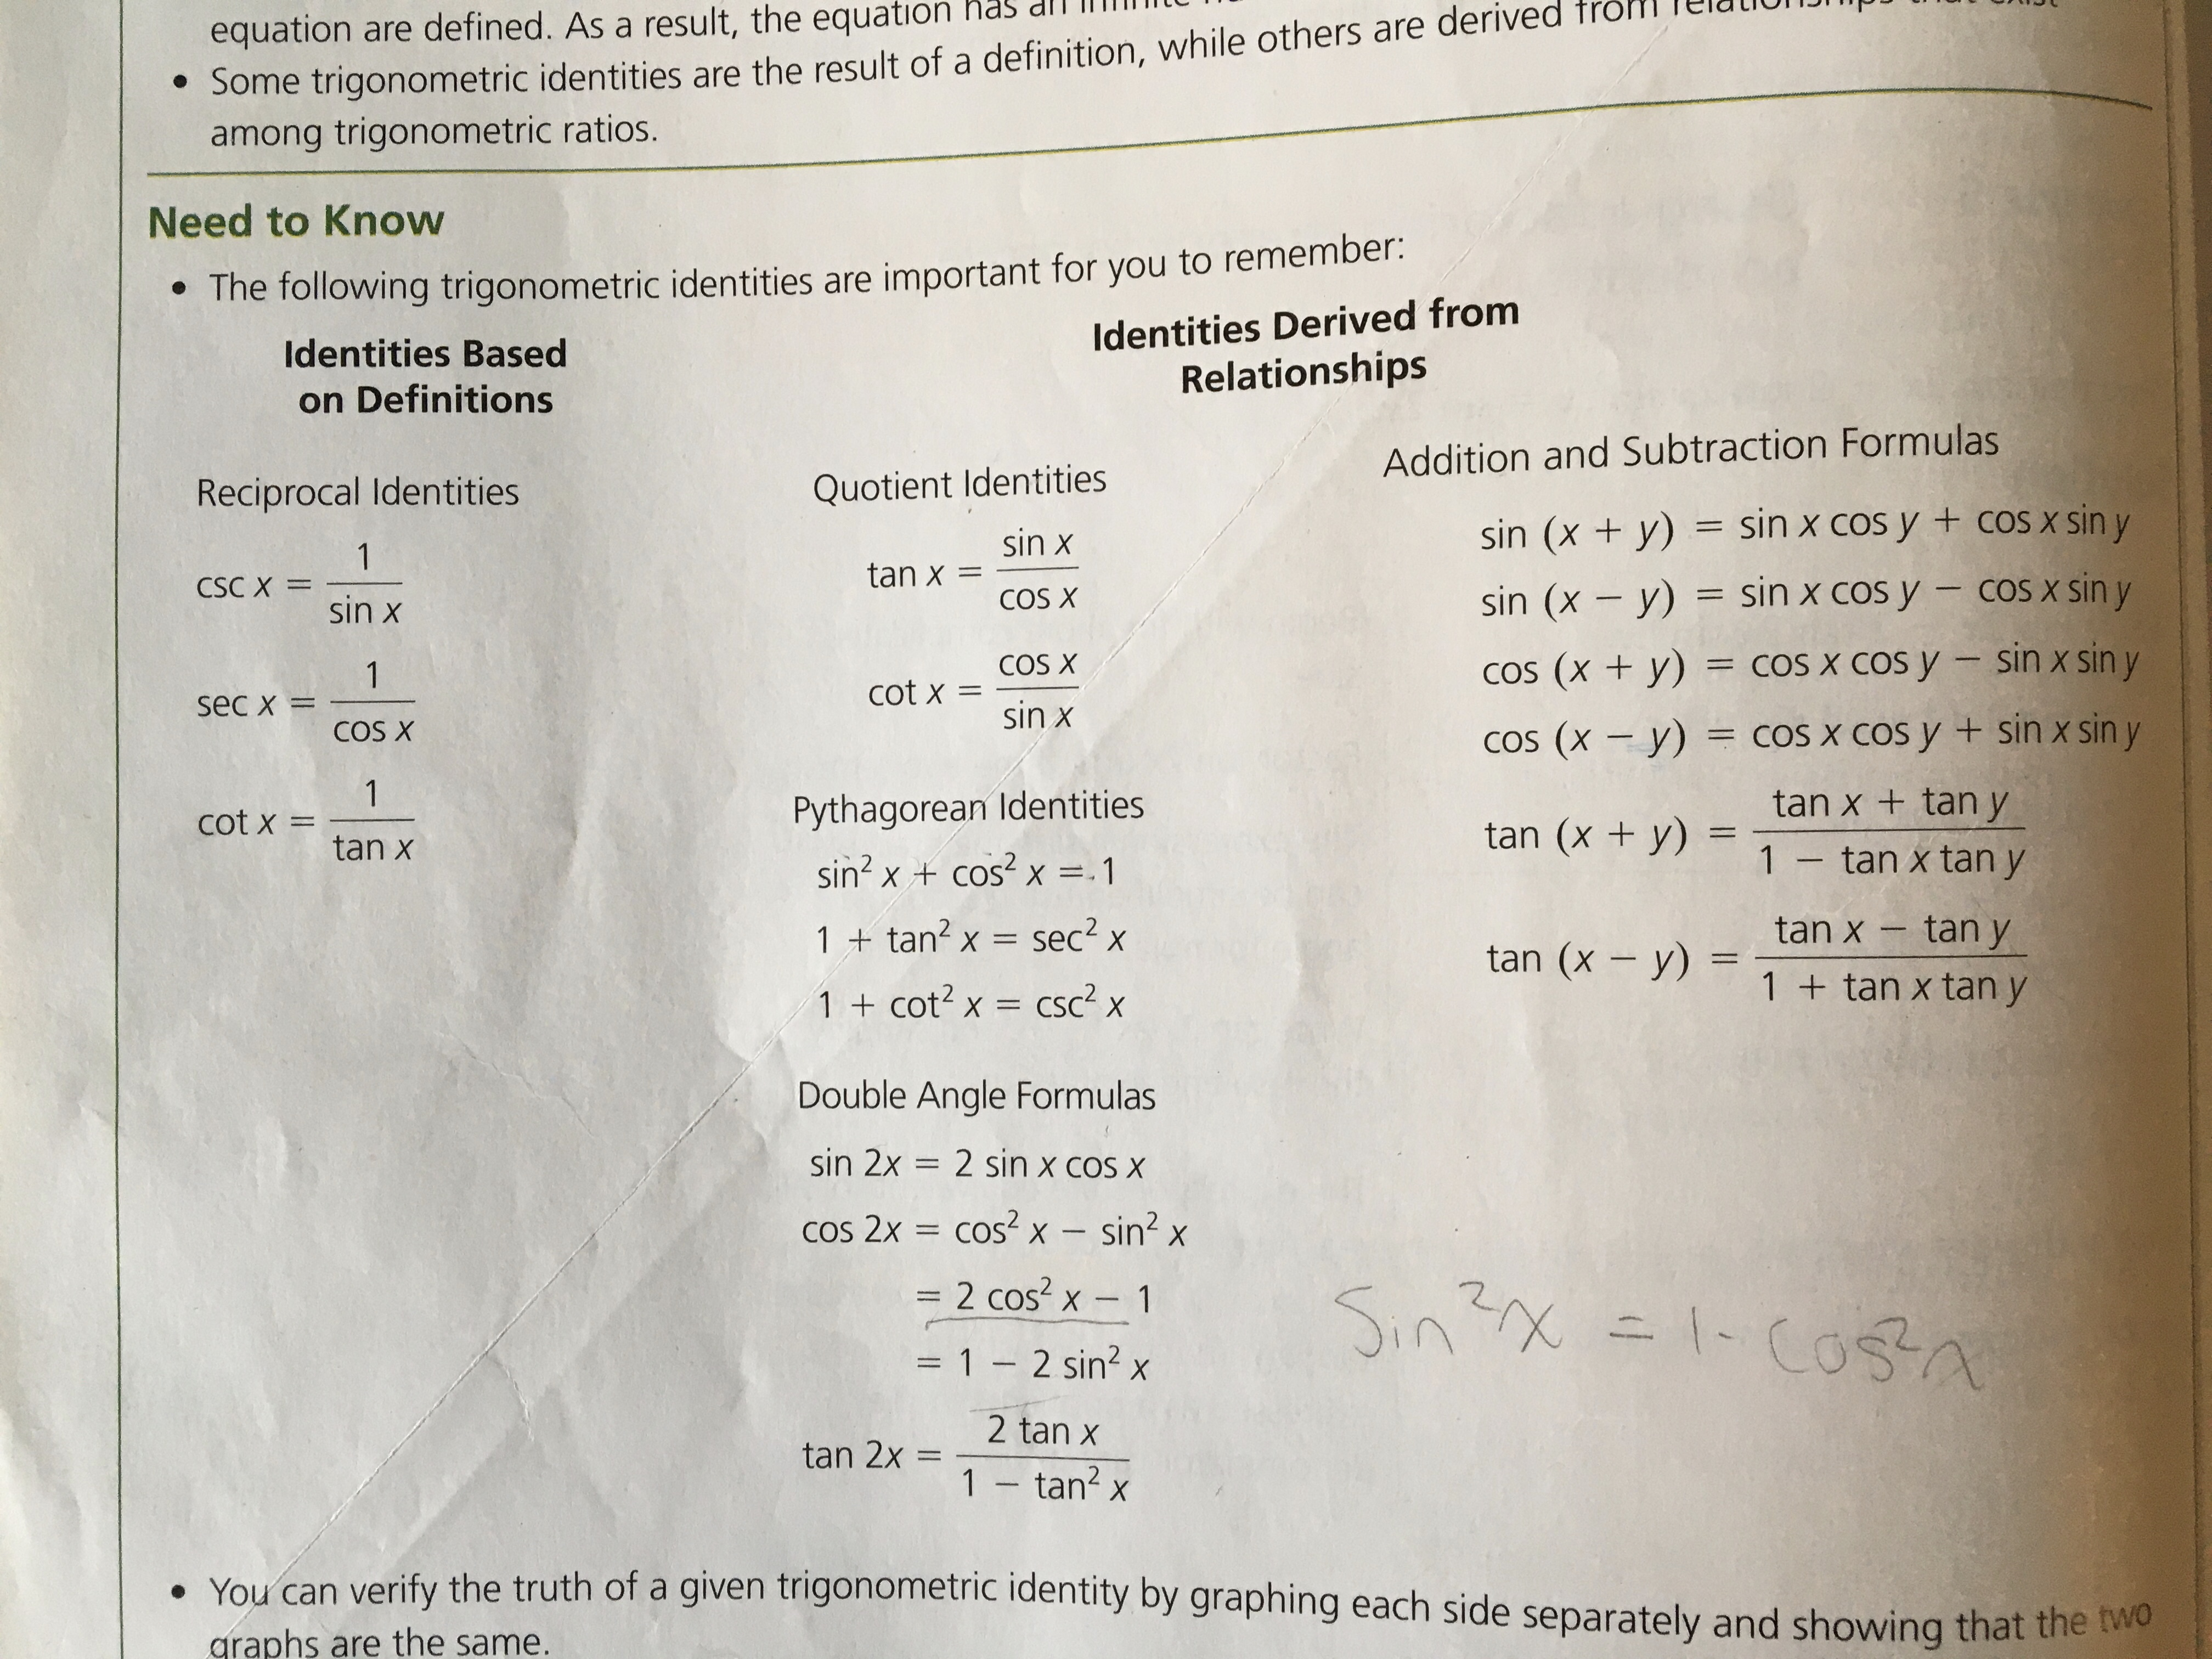
\includegraphics[width=\linewidth]{IMG_0836.JPG}

    \subsection{Solve Linear Trig Equations}
    \begin{itemize}
        \item Solve linear trig equations like regular linear Equations
        \item Be wary of the periodic nature of the relationship, can have multiple solutions within the interval given
    \end{itemize}

    \subsection{Solve Quadratic Trig Equations}
    \begin{itemize}
        \item WARNING: WEAK IN THIS AREA 
        \item Can be solved initially algebraicly
        \item Can have multiple solutions, some are extraneous
        \item Usually factor first before solving
    \end{itemize}

    %Chapter 8
    \section{Chapter 8: Logarithmic Functions}

    \subsection{Exploring Logarithms}
    \begin{itemize}
        \item Logarithms is the inverse of exponents
        \item the logarithmic form of $y = a^x$ is $x = \log_a y$
        \item The y axis acts as asymtotes
        \item x and y intercept is 1
        \item D:$\{ x \in R \mid x > 0 \}$, R:$\{ y \in R \}$
    \end{itemize}

    %graphc
    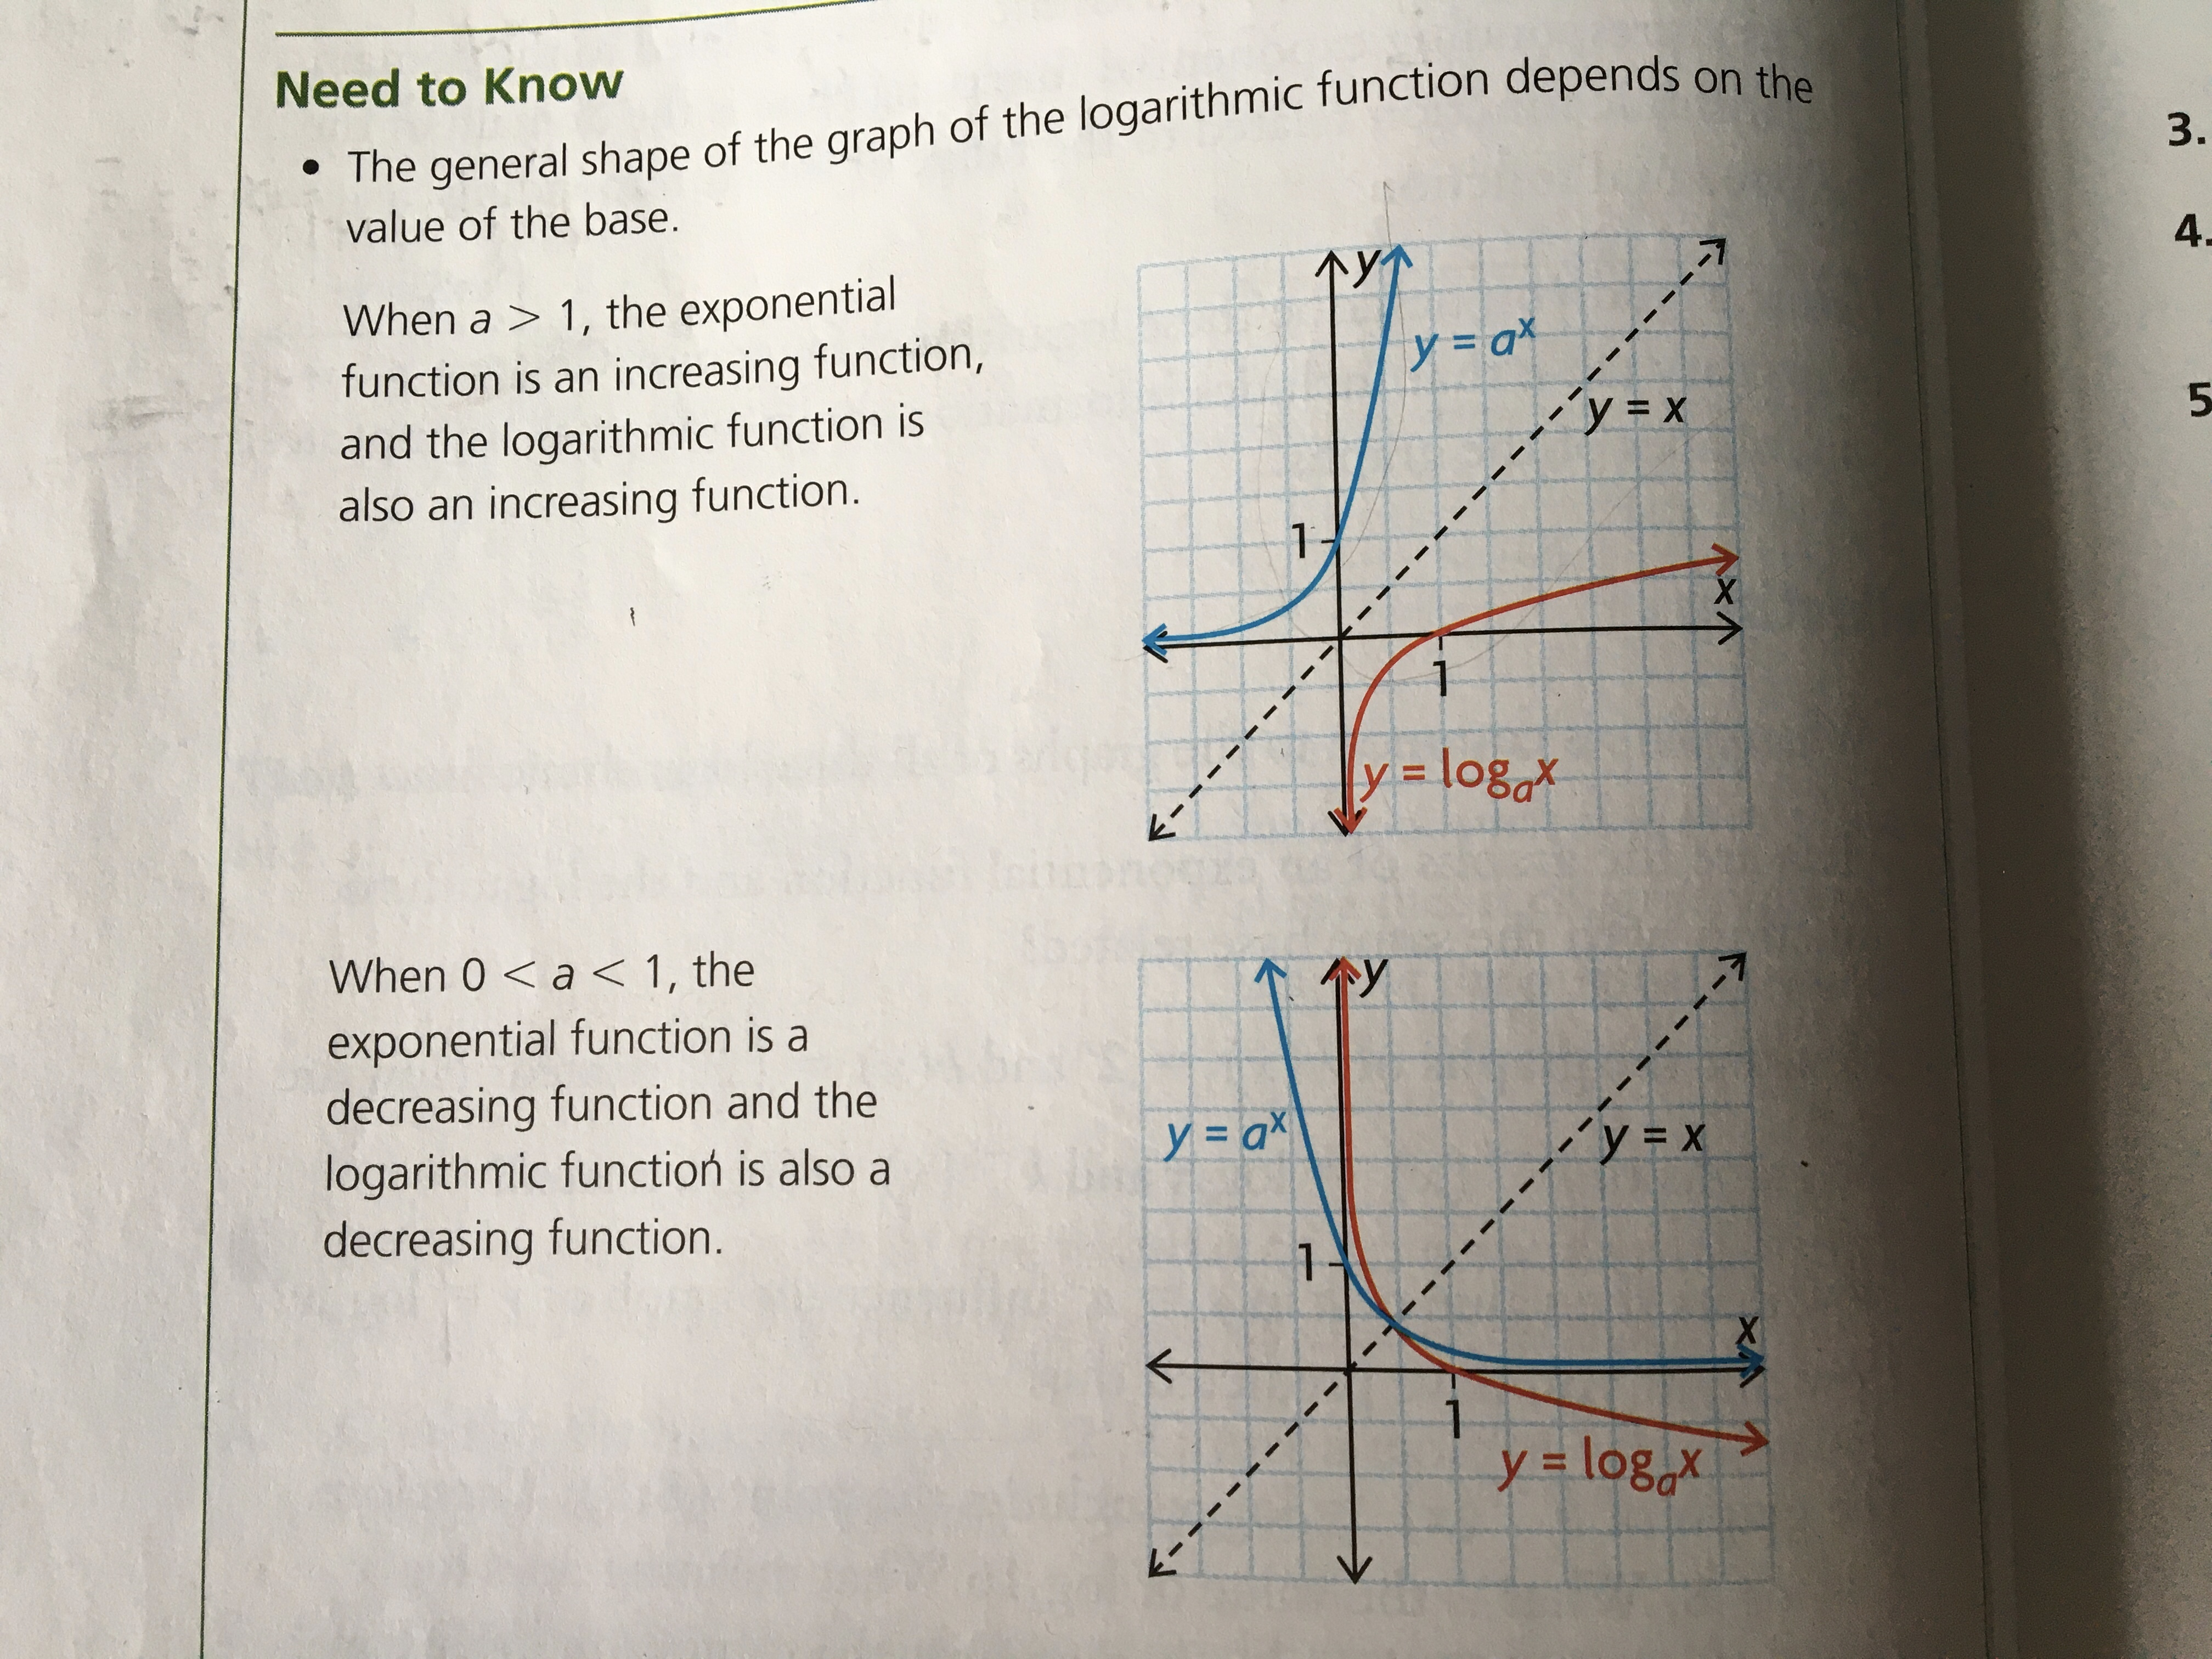
\includegraphics[width=\linewidth]{IMG_0837.JPG}

    \subsection{Transformations}
    \begin{itemize}
        \item Like exponential transformations
        \item $f(x) = a \log_{base}(k(x-d))+c$
        \item \textbf{transformations of parent functions}
        \begin{itemize}
            \item $|a|$ gives vertical stretch or compression, a gives reflection
            \item $\frac{1}{|k|}$ gives horizontal stretch or compression, k gives reflection
            \item d and c give h and v translations
        \end{itemize}
    \end{itemize}

    \subsection{Evaluating Logs}
    \begin{itemize}
        \item Can be solved in many ways
        \item Can rewrite in exponents
        \item Rewrite in log form and simplify
        \item Log of negatives does not exist
        \item properties:
        \begin{itemize}
            \item $log_a1=0$
            \item $log_aa^x=x$
            \item $a^{log_ax} = x$
        \end{itemize}
    \end{itemize}

    \subsection{Laws of Logarithms}
    \begin{itemize}
        \item Directly related to exponent laws
        \item When a, x, y $>$ 0 and a $\neq$ 1
        \begin{itemize}
            \item product law: $\log_axy = \log_ax + \log_ay$
            \item quotient law: $\log_a \frac{x}{y} = \log_ax - \log_ay$
            \item power law: $\log_ax^r = r \log_ax$
        \end{itemize}
    \end{itemize}

    \subsection{Solving Exponential Equations}
    \begin{itemize}
        \item if $a^m = a^n, m = n$ where $a > 0, a \neq 1 and m, n \in R$
        \item if $\log_aM = \log_aN, M = N$ where $ M, N > 0, a > 0, a \neq 1$
        \item ``To solve the exponential equation algebraically, take base 10 logs of both sides and use power rule to simplify before solving for unknown var"
    \end{itemize}

    \subsection{Solvng Logarithmic Equations}
    \begin{itemize}
        \item Can be expressed in exponential form 
        \item Can be simplified with log/exp laws
        \item Dont forget to check for inadmissable solutions
    \end{itemize}

    \subsection{Application}
    \begin{itemize}
        \item Log 10 helps to compare a scale that accelerates rapidly
    \end{itemize}

    \subsection{Rates of Change}
    \begin{itemize}
        \item ROC is not constant
        \item instantaneous roc can be take using estimate linear tangents
        \item estimate using greatest and least roc
    \end{itemize}

    %Chapter 9
    \section{Chapter 9: Combinations of Functions}

    \subsection{Exploring}
    \begin{itemize}
        \item New functions can be made by combining simple functions
        \item Done by regular operations: add, subtract, multiply, divide
        \item New characteristics are a combination of prev parent characteristics
    \end{itemize}

    \subsection{Sum and Difference}
    \begin{itemize}
        \item When f(x) and g(x) are combined, they become the sum $(f+g)(x)$ or difference $(f-g)(x)$ of f and g
        \item Y (output) values are combined
        \item $(f + g)(x) = f(x) + g(x)$
    \end{itemize}

    \subsection{Product}
    \begin{itemize}
        \item $f(x) \times g(x)$ creates a product formula: $(f\times g)(x)$
        \item Graph result by multiplying y value
    \end{itemize}

    \subsection{Quotient}
    \begin{itemize}
        \item Same thing, just divide functions and y results
    \end{itemize}

    \subsection{Composition}
    \begin{itemize}
        \item Composite functions is a where one function lies within another function
        \item $f(g(x)) = (f\circ g)(x)$
    \end{itemize}

    \subsection{Solving}
    \begin{itemize}
        \item Can be solved by finding the unknown value
        \item try to rearange to equal zeroe
        \item Be careful of $>$ vs $\geq$
    \end{itemize}

    \subsection{Modelling}
    \begin{itemize}
        \item Use a model in order to give an approximate representation of a real life relationship
        \item Increasing data increases points, increases accuracy
        \item Function chosen should make sense in the situations
    \end{itemize}

    %Chapter 2
    \section{Chapter 2: Rates of Change}

    \subsection{Determining Average ROC}
    \begin{itemize}
        \item essentielly change in y / change in x
        \item $\frac{f(x_2) - f(x_1)}{x_2-x_1}$
        \item The slope of the line passing through the 2 points
    \end{itemize}

    \subsection{Instantaneous ROC}
    \begin{itemize}
        \item Average raote of change at close to a single point, a Tangent
        \item Calculate by getting 2 points that are very close or equal to the point chosen
    \end{itemize}

    \subsection{Istantaneous ROC Graphs}
    \begin{itemize}
        \item Slope = ROC
    \end{itemize}

    \subsection{Creating Graphical Models}
    \begin{itemize}
        \item Can be used to express distance over time \rt speed
    \end{itemize}

    \subsection{Solving Problems}
    \begin{itemize}
        \item Zero at the peaks and troughs of curves
        \item if negative or positive, will trend downwards or upwards
    \end{itemize}

\end{document}